\chapter{Liquid Argon Detectors at the Intensity Frontier}\label{ch:1}


In the next few years, LArTPC experiments -- such as the Short-Baseline Neutrino program (SBN) and DUNE -- will be major players in the intensity frontier field. 


\section{Liquid Argon Time Projection Chambers at the Intensity Frontier}

%Bubble-chamber experiments played a key role in probing the properties of ?-interactions. The Liquid Argon Time Projection Chambers (LArTPC) technology,  first proposed by C.Rubbia in 1977 with ICARUS project [14], is considered the modern evolution of bubble-camber concept, with the additional features of three-dimensional event reconstruction, high-resolution calorimetry, active mass coincident with detector sensitive mass and can intrinsically supply a trigger signal (self-triggering) by means of the scintillation light produced in the liquid noble gas. This technology is ideal to perform $\nu$-studies in a broad energy range, from MeV up to few GeV, with high event reconstruction efficiency, thanks to the capability of particle identifcation and detailed reconstruction of different interaction topologies. In Figure 1.4 is shown a neutrino interaction event, producing a proton, a pion and a muon, as seen in a bubble chamber and in a LArTPC.


\subsection{Time Projection Chamber}
\subsection{Ionization Detectors with Noble Liquids}
\subsection{LArTPC: Principles of Operation}
\subsection{Liquid Argon Ionization Charge Detection}
\subsubsection{Electron Life Time \& purity}
\subsubsection{Space Charge Effect}
\subsubsection{Recombination Effect}
\subsection{Liquid Argon scintillation Light Detection}
\subsubsection{LAr Scintillation Process}
\subsubsection{Wavelength Shifting of LAr Scintillation Light}
\section{The SBN Program: Neutrino Interaction and Detection}
%\subsection{SBN Goals}
%\subsection{Neutrino Interactions and Detection }
\section{DUNE: Rare Decay Searches}
The key elements for a rare decay experiment are: massive active volume, long exposure, high identification efficiency and low background. 
%The limit to proton lifetime in case of absence of signal and backgrounds is set by calculating
%$$\tau/B > M\times \epsilon\times T \times 10^{32},$$ 
%where M is the detector mass in kton, $\epsilon$ the signal detection efficiency after cuts to suppress backgrounds (dependent on the considered decay mode), T is the exposure in years, B the assumed branching fraction for the considered mode and  $10^{32}$ is a factor accounting for the number of nucleons in a kton of material \cite{Bueno2007}.
Figure \ref{fig:PDKExperimentalLImit} shows the current best experimental limits on nucleon decay lifetime over branching ratio (dots). Historically, the dominant technology used in these searches has been water Cherenkov detectors: all the best experimental limits on every decay mode are indeed set by Super-Kamiokande \cite{PhysRevD.90.072005,PhysRevLett.115.121803}.  It is particularly important to notice that the kaon energy for the proton decay mode $p \rightarrow K^+ \bar{\nu}$ is under Cherenkov threshold.  Super-Kamiokande set the limit on the lifetime for the $p \rightarrow K^+ \bar{\nu}$ mode by  relying exclusively on photons from nuclear de-excitation. For this reason, an attractive alternative approach to identifying nucleon decay is the use of a Liquid Argon Time Projection Chamber (LArTPC). 

LArTPCs can complement nucleon decay searches in modes where water Cherenkov detectors are less sensitive, especially $p\rightarrow K^+\bar{\nu}$. According to \cite{Acciarri:Dune}, DUNE will have an active volume large enough, have sufficient shielding from the surface, and will run for lengths of time sufficient to compete with Hyper-K, opening up the opportunity for the discovery of nucleon decay. 

\begin{figure}[hbpt]
\centering
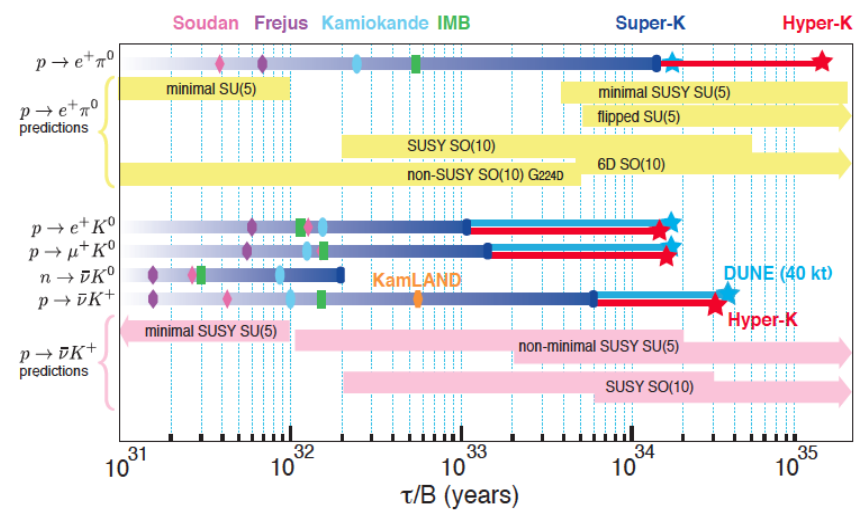
\includegraphics[width=6.5in]{Chapter-2/Images/PDKExperimentalLImit.png}
\caption{Proton decay lifetime limits from passed and future experiments.}
\label{fig:PDKExperimentalLImit}
\end{figure}


\begin{figure}[hbpt]
\centering
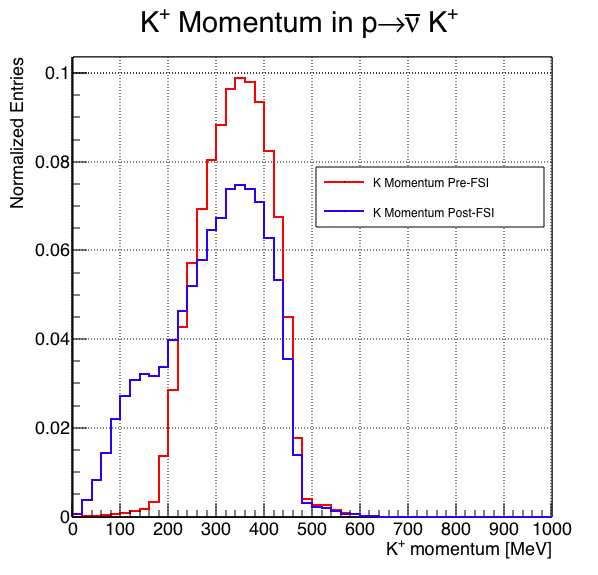
\includegraphics[width=3.5in]{Chapter-2/Images/pdkGenie.png}
\caption{Momentum of the kaon outgoing a proton decay event as simulated by the Genie 2.8.10 event generator in argon. The red line represent the kaon momentum distribution before undergoing the simulated final state interaction inside the argon nucleus, while the blue line represents the momentum distribution after FSI. }
\label{fig:PDKGENIE}
\end{figure}


%\subsection{Non-Accelerator Physics Program}
%\subsection{Rare Decay Searches: Experimental Limit}
%\subsection{Nucleon Decay Detection in LAr}
\section{Enabling the next generation of discoveries: LArIAT}
LArIAT, a small Liquid Argon Time Projection Chamber (LArTPC) in a test beam,  is designed to perform an extensive physics campaign centered on charged particle cross section measurements while characterizing the detector performance for future LArTPCs. LArTPC represents one of the most advanced experimental technologies for physics at the Intensity Frontier due to its full 3D-imaging, excellent particle identification and precise calorimetric energy reconstruction. This complex technology however needs a thorough calibration and dedicated measurements of some key quantities to achieve the precision required for the next generation of discoveries at the Intensity Frontier which LArIAT can provide. 

The LArIAT LArTPC is deployed in a dedicated calibration test beamline at Fermilab.
We use the LArIAT beamline to characterize the charge particles before they enter the TPC: the particle type and initial momentum is known from beamline information. The precise calorimetric energy reconstruction of the LArTPC technology enables the measurement of the total differential cross section for  tagged hadrons. 
The Pion-Nucleus and Kaon-Nucleus total hadronic interaction cross section have never been measured before in argon and they are a fundamental step to shed light on light meson interaction in nuclei. Additionally, these measures provides a key input to neutrino physics and proton decay studies in future LArTPC experiments like SBN and DUNE.
\textcolor{red}{add paragraph on all wonderful things lariat can do... some event displays would be nice!}



\textcolor{red}{ADD genie proton decay kaon distribution and lariat beamline overlaied}
The signature of a proton decay event in the ``LAr golden mode" is the presence of a single kaon of about 400 MeV in the detector. 
